In this chapter, Redis performance in terms of latency, throughput and system resource requirements is examined. Initially, we will focus on performance under the default configuration of Redis. Subsequently, the scalability characteristics of Redis are explored. Focus is given to the impact of multiple Redis instances running simultaneously on the same machine under various levels of workload.

Unless otherwise stated, all benchmarks are performed to target the required Quality of Service (QoS) of achieving 99th percentile latency under 1 millisecond.


\section{Out of the Box Performance}
\label{sec:redis-default}
Firstly, in order to understand the baseline performance of Redis we consider the default configuration of Redis. A Redis deployment can be started with the following command:
\begin{lstlisting}
redis redis.conf --port 11120
\end{lstlisting}

By default, a Redis deployment comes with a default configuration file \texttt{redis.conf}\cite{RedisConfiguration}. Any options specified in the configuration file can be overridden from the command line by prefixing them with \texttt{--}, in our case we are overriding the port number and setting it to 11120. All other configuration options remain unmodified.

In order to understand the default Redis performance, we design the benchmark to exert an increasing level of load on the Redis server. Initially, we start with 2 threads and 1 connection per each thread on all workload generating clients, there are 7 such clients in our setup.  In our workload, we define the key space to be up to 100 million keys with an object size of 64 bytes yielding around 6.4 GB of data while the memory capacity of the server is 8GB and therefore data should not be swapped out of main memory. The workload generating clients are executed with the following command:

\begin{lstlisting}
memtier -s nsl200 -p 11120
    -c <connection_count> -t 2
    -P redis
    --random-data --data-size=64
    --key-minimum=1 --key-maximum=100000000
    --test-time=400
\end{lstlisting}

The number of connections per each thread is increased linearly in each subsequent benchmark run. Each workload is executed over the course of 400 seconds and the data is randomly generated with keys drawn from a uniform distribution between 1 and 100 million.


\subsection{Latency vs Throughput}

\begin{figure}[h]
    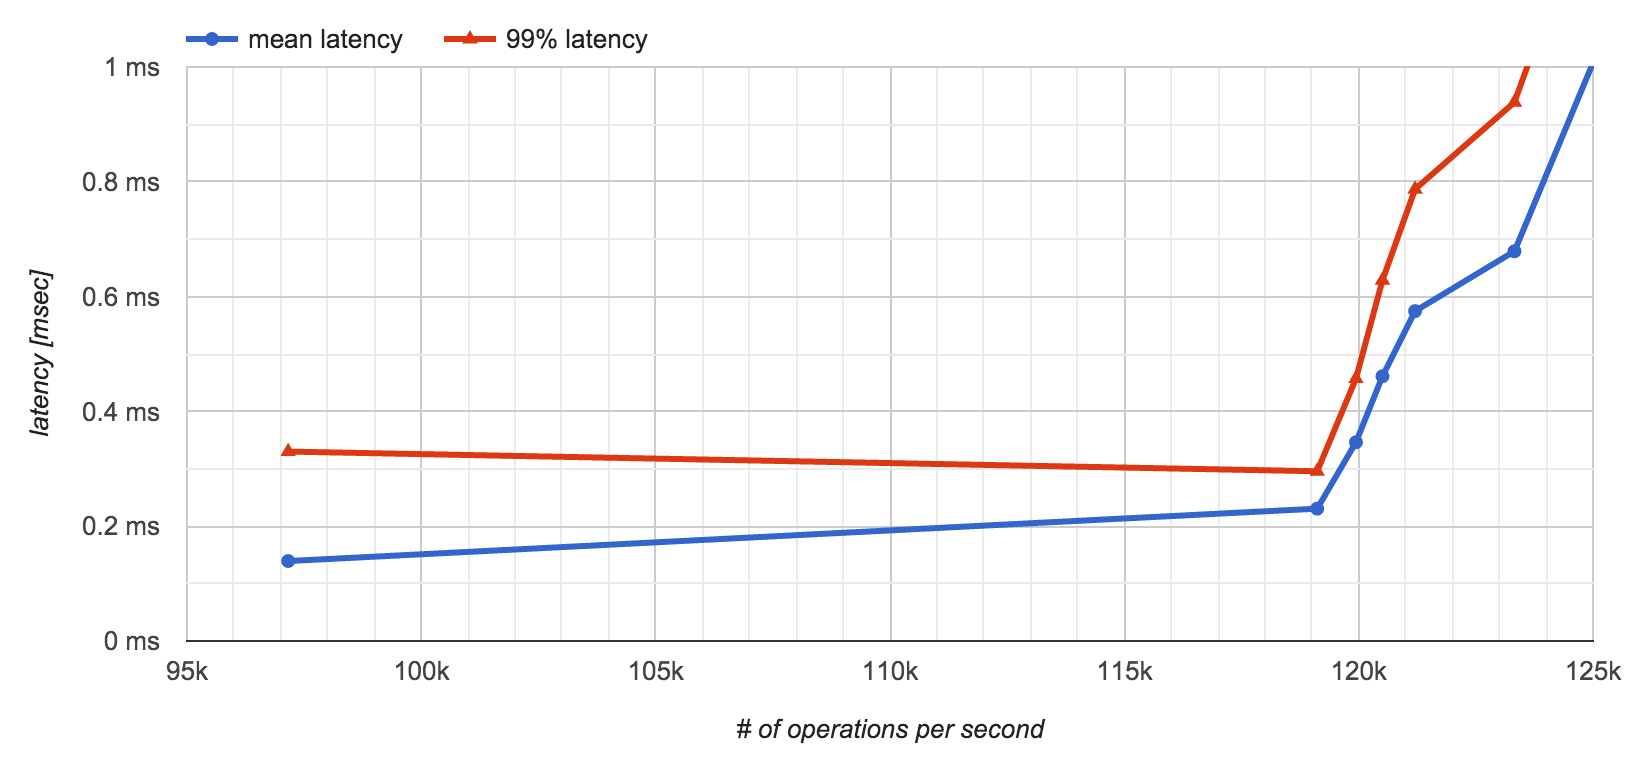
\includegraphics[width=\textwidth]{./res/6_default_latency_ops.png}
    \caption{Redis: Throughput vs Mean and 99th percentile latency}
    \label{fig:redis-default-latency-ops}
\end{figure}

Figure \ref{fig:redis-default-latency-ops} plots the relationship between mean latency and the 99th percentile latency on the vertical axis and the number of operations per second on the horizontal axis. The graph has been trimmed to show only data which satisfies the QoS requirements.

We can observe that the number of operations Redis processes increases steadily until it reaches 119k requests per second at which point a further increase in throughput comes at a disproportionately grater cost in both mean and 99th percentile latency. The peak throughput observed under the QoS requirements is around 123k requests per second.


\subsection{CPU Utilization}

\begin{figure}[h]
    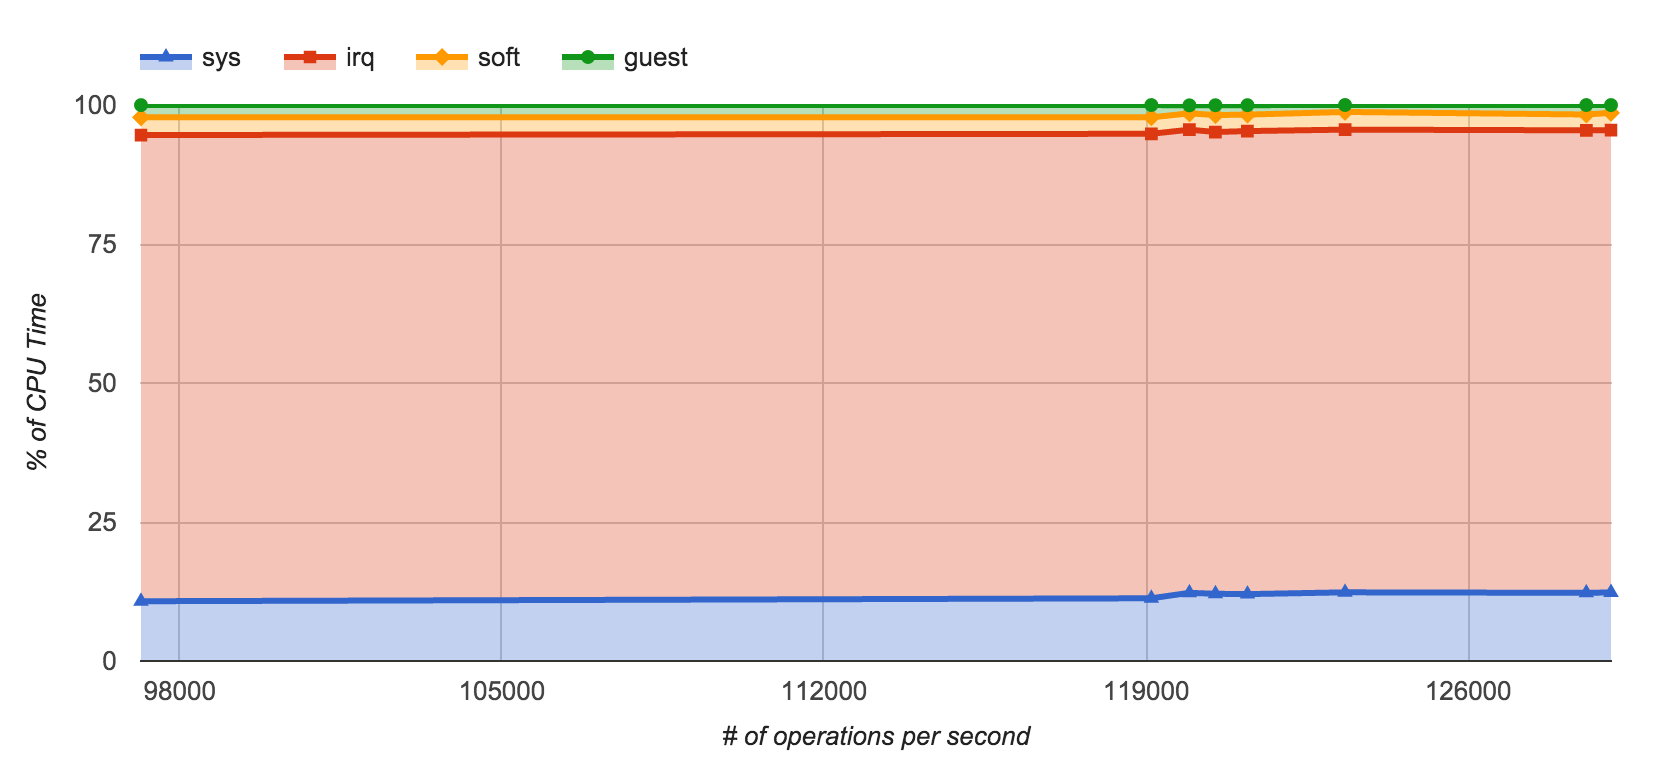
\includegraphics[width=\textwidth]{./res/6_default_cpu.png}
    \caption{Redis: CPU Utilization}
    \label{fig:redis-default-cpu}
\end{figure}

Figure \ref{fig:redis-default-cpu} outlines the CPU utilization in terms of time spent processing system calls (sys), servicing hardware interrupts (irq), handling software interrupts (soft) and processing related to Redis (guest).

We can observe that servicing hardware interrupts consumes the majority of the processing time - 83 percent. This is the result of receiving and dispatching a large number of requests through the NIC. The amount of CPU time devoted to processing system calls is about 10 percent while processing software interrupts accounts for 3 percent. Redis itself requires only about 2 percent of the overall CPU time.

Redis appears to be network constrained rather than CPU constrained in the workload examined above. This is reasonable as Redis is executing within one main event loop therefore it does not require locking and does not generate heavy load on the CPU when looking values up in the cache.


\section{Multiple Redis Instances}
\label{sec:multiple-redis-instances}

As seen in section \ref{sec:redis-default}, Redis cannot increase overall throughput of the system with only a single instance as only a single core is capable of processing requests and becomes the bottleneck. An immediate solution to this problem is to provision a larger number of instances on a multi-core system in order to better utilize the hardware resources.

In this benchmark, we examine the effects increased number of Redis instances with respect to latency, 99th percentile latency and overall throughput of the system. Additionally, we examine the effect of multiple instances on the CPU usage.

Firstly, multiple instances of Redis can be spawned easily on the server by binding them to distinct port numbers. Out of the box, Redis does not provide the capability to proxy multiple instances of Redis through a single port in order to load balance the instances. There is the option to configure a Redis cluster, however, the intended use case is primarily for resiliency and fail over. In this benchmark, we consider a simpler scenario where each instance is isolated from each other and acts as an independent cache. This is a simplification of a real world scenario, however, a large deployment of Redis could be designed to partition the key space and utilize multiple independent instances similarly. The Redis application can be spawned with the following script:

\begin{lstlisting}
for i in [1..n]
    redis-server redis.conf --port (11120 + i) --maxmemory (6 / i)gb
\end{lstlisting}

Note that we are explicitly specifying the maximum amount of memory each instance will be allocated. In our case, we partition 6 GB of memory space evenly between the individual instances.

Secondly, in order to obtain comparable results, the load exerted on the Redis cache must remain constant. The load itself, however, needs to be partitioned across all of the instances of Redis evenly. In order to achieve this, each workload generating client spawns \texttt{i} instances of the benchmark and targets its respective Redis instance. We use the following script to start the workload generating clients:

\begin{lstlisting}
for i in [1..n]
    memtier -s nsl200 -p 11120
        -c round(16 / i)
        -t 1
        -P redis
        --random-data --data-size=64
        --key-minimum=1 --key-maximum=round(100000000 / i)
        --test-time=400
\end{lstlisting}

Initially, we start with 16 connections and 1 thread. As we increase the number of instances, the number of connections goes down, however, a larger number of instances are deployed. Note that we are using a \texttt{round} function to ensure that the number of connections as well as the maximum key are integers. In order to smooth out load variance caused by integer divisibility, we consider two cases. One in which the \texttt{round} function is defined as the \texttt{ceiling} function and the other when it is defined as the \texttt{floor} function. The results of both types of the \texttt{round} function are then averaged. If a higher number of workload generating clients were available for the experimentation, the round approach would not be required.

Furthermore, the generated dataset is 6.4GB (100 million keys * 64 bytes of data). This is by design and should lead to evictions in the cache as the size approached the maximum.


\subsection{Number of Instances vs Latency and Throughput}

\begin{figure}[h]
    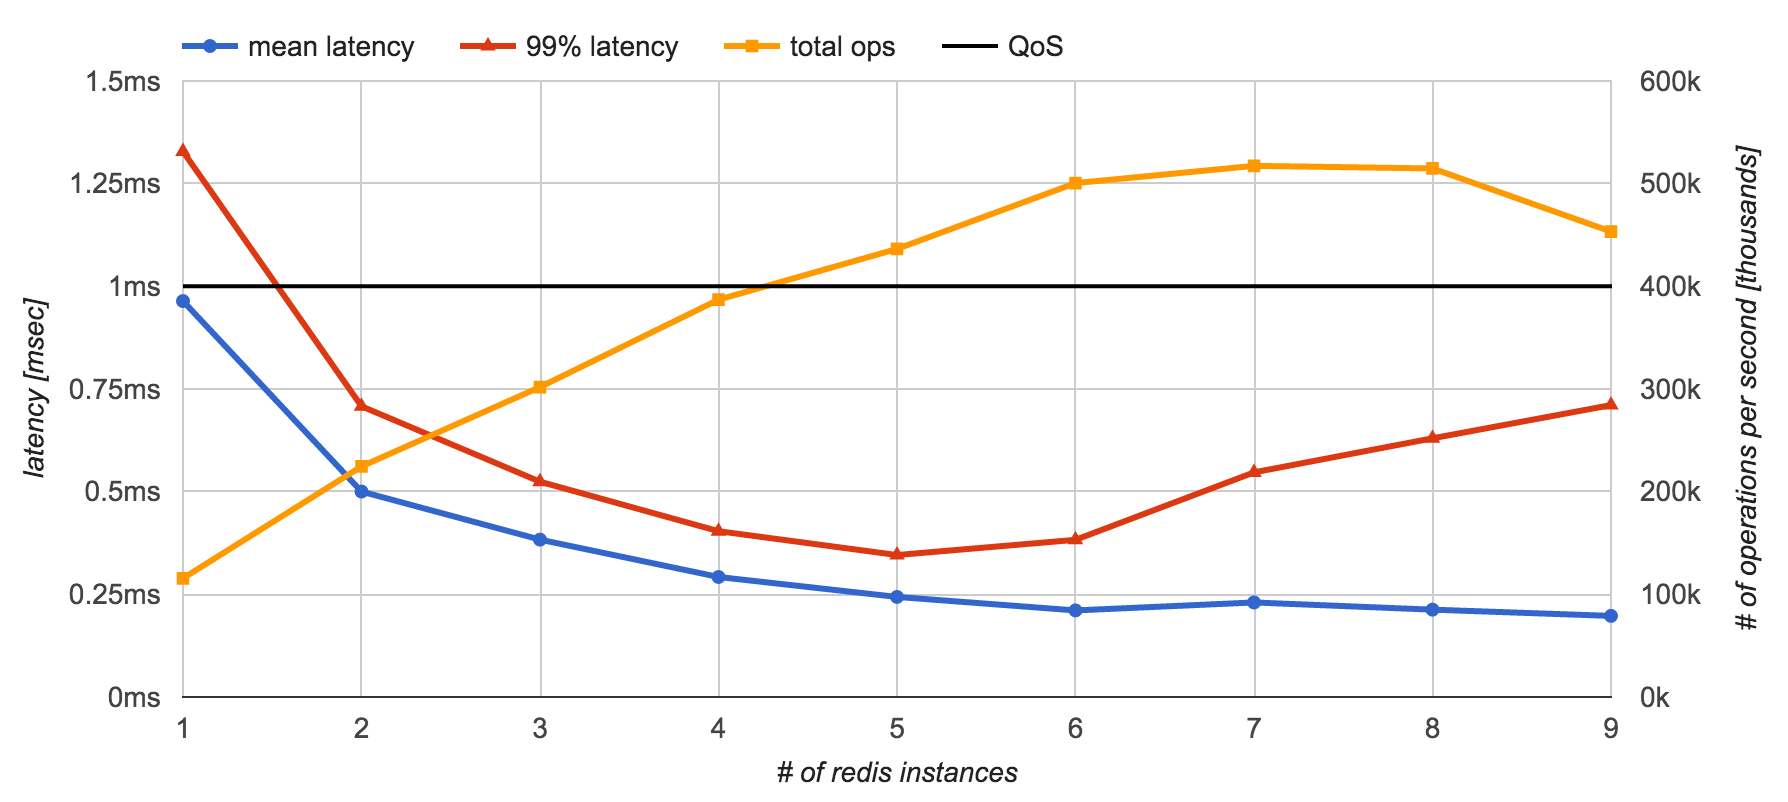
\includegraphics[width=\textwidth]{./res/6_instances_latency_ops.png}
    \caption{Redis Instances: Latency, Throughput vs Number of instances}
    \label{fig:redis-instances-latency-ops}
\end{figure}

Figure \ref{fig:redis-instances-latency-ops} plots the relationship between the number of Redis instances running simultaneously on the cache server against the mean and 99th percentile latency on the left vertical axis and the total number of operations per second on the right axis. The black line positioned at 1ms outlines the QoS target of the benchmark.

As the number of processes increases, both mean and 99th percentile latency decrease steadily. The 99th percentile latency reaches a minimum at 5 processes and rises as number of processes is increased further. The minimum 99th percentile latency achieved is around 0.345ms. The mean continues to decrease at a much slower pace beyond it's minimum at 6 processes.

Additionally, as the number of instances increases, throughput increases. Throughput increases linearly until 6 instances are reached at which point the rate of increase decreases. Beyond 8 instances, the throughput begins to decrease. Between 6 and 8 instances, we are able to achieve close to 500k requests per second.

The QoS target is achieved in all but the 1 instance scenario. Furthermore, we can observe that Redis manages to scale quite well by increasing the number of instances until we reach 6 instances. Beyond 6 instances, the throughput degrades and the 99th percentile begins to climb again. The best balance of throughput and minimal 99th percentile latency is when running 6 instances, the same as the number of CPU cores available.

\subsection{CPU Utilization vs Instance Count}
Let us now explore the impact of running multiple Redis instances simultaneously on the CPU utilization.

\begin{figure}[h]
    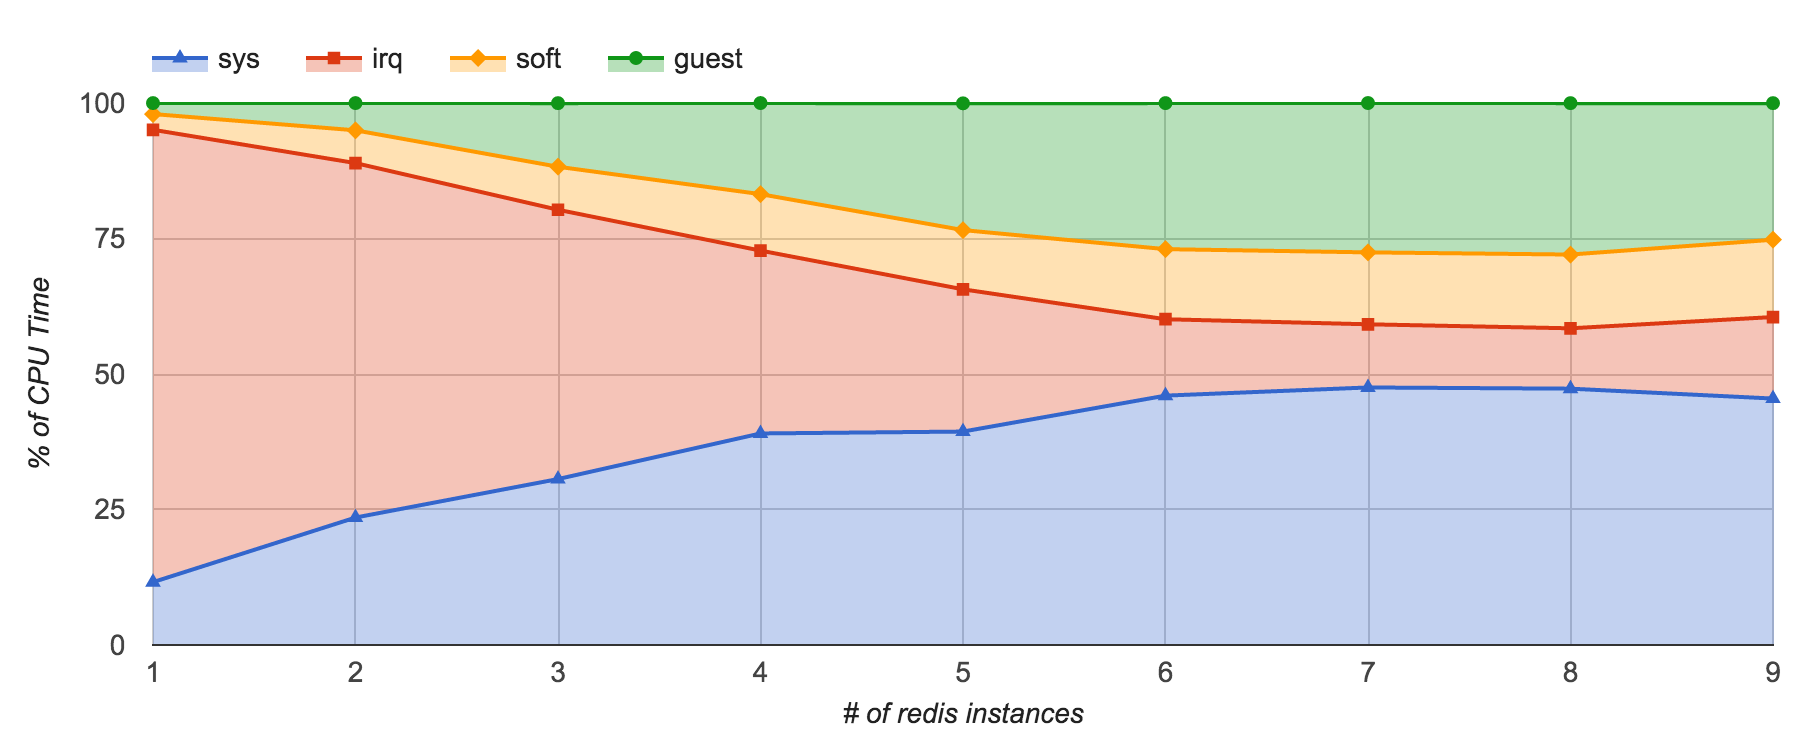
\includegraphics[width=\textwidth]{./res/6_instances_cpu.png}
    \caption{Redis Instances: CPU Utilization vs Number of Instances}
    \label{fig:6_instances_cpu.png}
\end{figure}

From \ref{fig:6_instances_cpu.png} we can see that as we increase the number of instances, the CPU usage of Redis (\textit{guest}) increases until we reach 6 instances at which point it flattens out. Similarly, the resources required by OS (\textit{sys}) to support the increasing number of instances grows until 6 processes, further increase in the number of instances does not result in increased resource usage. The amount of context switching (soft) required increases as the number of instances increases and remains constant beyond 6 instances. Conversely, the time spent processing hardware interrupts from the network decrease, this is due to batching at the network layer as the number of instances increases.

Despite the increased resource requirements by Redis, it still only accounts for about 27 percent CPU usage at 6 processes with majority of the CPU time spent in the operating system and or networking.


By spawning multiple instances of Redis, we have been able to dramatically increase the overall performance of the server. The peak throughput observed is at 500k requests per second while the mean and 99th percentile latency remains within the QoS restrictions.


\section{Pinned Redis Instances}

In the previous section we have observed that the performance of a Redis server can be greatly increased by spawning multiple Redis instances simultaneously. Pinning processes to distinct cores is suggested to improve tail latency \cite{leverich2014reconciling}. In this section, we examine the effect process pinning has on the performance of Redis. A Redis thread can be pinned to a unique core through the use of \texttt{taskset} utility as follows:

\begin{lstlisting}
taskset -pc <redis_pid> <core_id>
\end{lstlisting}

The Redis and benchmark configuration used is the same in section \ref{sec:multiple-redis-instances}, that is, the number of Redis processes is linearly increased while maintaining the same level load.

\begin{figure}[h]
    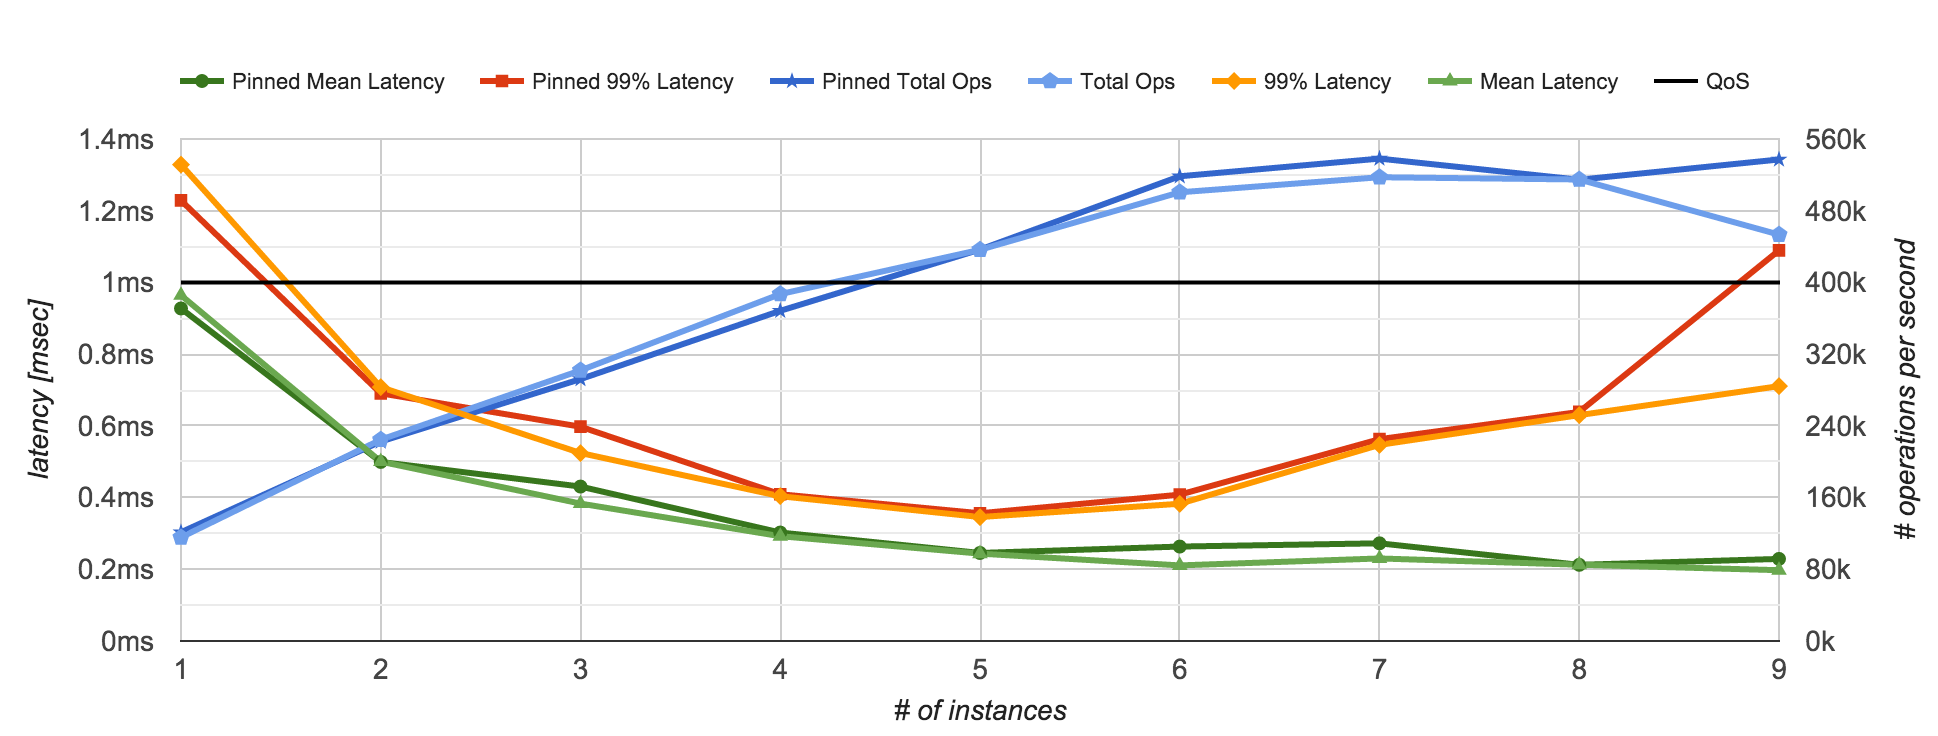
\includegraphics[width=\textwidth]{./res/6_pinned.png}
    \caption{Redis Instance Pinning: Instances vs Latency and Throughput}
    \label{fig:6_pinned.png}
\end{figure}